% -----------------------------------------------
% Template for JIM
%     jim.sty -> style file
% By Eloi Batlle (eloi@iua.upf.es), changes for 
% ICMC by Bram de Jong (bdejong@iua.upf.es)
% changes for JIM 2007 by Dominique Fober (fober@grame.fr)
% changes for JIM 2009 by Olivier Tache (olivier.tache@imag.fr)
% -----------------------------------------------

\documentclass{article}
\usepackage{jim,amsmath}
\usepackage[utf8]{inputenc}
\usepackage[francais]{babel}
\usepackage[T1]{fontenc}
%\usepackage{pxfonts}
\usepackage{graphicx}
\usepackage{balance}
\usepackage{ifpdf}
\usepackage{hyperref}

\usepackage{verbatim}
\usepackage{color}
\usepackage{textcomp}

\definecolor{mygrey}{gray}{0.93}
\definecolor{figOrange}{RGB}{212,85,0}
\definecolor{figRed}{RGB}{128,0,0}
\definecolor{red}{RGB}{250,0,0}
\definecolor{figBlue}{RGB}{0,136,170}

\newenvironment{ExprCode}	{\vspace{-2mm} \small\verbatim}{\endverbatim\vspace{-2mm}}
\newcommand{\OSC}[1]	{{\fontsize{10pt}{10pt} \selectfont\texttt{#1}}}
\newcommand{\oper}[1]	{\textcolor{figRed}{#1}}
\newcommand{\param}[1]	{\textcolor{figOrange}{#1}}
\newcommand{\prefix}[1]	{\textcolor{figBlue}{#1}}

\newcommand{\note}[1]{\textcolor{red}{(#1)}}


\newcommand{\sExpr}{\emph{score expression}}
\newcommand{\sExprs}{\emph{score expressions}}
\newcommand{\SExpr}{\emph{Score expressions}}
\newcommand{\lowTilde}{\texttildelow}
\newcommand{\tab}{\hspace*{4mm}}

\let\olditemize\itemize
\let\oldenditemize\enditemize
\renewenvironment{itemize} 	{\olditemize \setlength{\itemsep}{1mm}}{\oldenditemize}

\newcommand{\sample}	[1]			{\vspace{-0.2em}\begin{center}\colorbox{mygrey}{\begin{minipage}[t]{0.97\columnwidth} {\small \texttt{#1}}\end{minipage}}\end{center}}


% Title.
% ------
\title{Composition de partitions symboliques dans INScore}

% Single \textsc{address}
% To use with only one author or several with the same address
% ---------------
\oneauthor
  {G. Lepetit-Aimon \qquad D. Fober \qquad Y. Orlarey \qquad S. Letz} {Grame \\
  Centre nationale de création musicale \\
  Lyon - France \\
     {\tt {\small \{gabriel.lepetit.aimon,fober,orlarey,letz\}@grame.fr}}}

% Two addresses
% --------------
%\twoauthors
%  {First author} {School \\ Department}
%  {Second author} {Company \\ Address}

% Three addresses
% --------------
%\threeauthors
%  {Auteur 1} {Organisme \\ Adresse électronique}
%  {Auteur 2} {Organisme \\ Adresse électronique}
%  {Auteur 3} {Organisme \\ Adresse électronique}

\begin{document}
%
\maketitle
%
\begin{abstract}
INScore est un environnement pour la conception de partition interactives augmentées, tourné vers des usages non conventionnels de la notation musicale. L'environnement permet d'utiliser et de composer des ressources graphiques arbitraires pour la représentation de la musique aussi bien que de la notation symbolique aux formats GMN (Guido Music Notation) ou MusicXML. INScore a été étendu pour fournir des opérations de composition de partitions en notation symbolique avec un jeu d'opérateurs qui de manière consistante, prennent des partitions en entrée pour produire une partition en sortie. L'API d'INScore inclut des \sExprs , aussi bien au niveau OSC que dans son langage de script. 
Le travail présenté est basé sur une recherche précédente qui a porté sur les problèmes de consistance de la notation musicale à travers des opérations de composition de partitions. Ce sont les aspects langage et stratégies d'évaluation des \sExprs\ qui sont abordés ici.
\end{abstract}

%==============================================================
\section{Introduction}\label{sec:introduction}

La notation musicale fait face à nombreux défis posés par la création contemporaine. Les musiques spatialisées, les nouveaux instruments, les partitions interactives et temps-réel, sont parmi les nouveaux domaines couramment explorés par les artistes. 
La notation musicale conventionnelle ne couvre pas les besoins de ces nouvelles formes musicales et de nombreuses recherches et approches ont récemment émergé, témoignant d'une certaine maturité des outils informatiques pour la notation et la représentation de la musique. Les problèmes posés par la spatialisation de la musique \cite{Ellberger_tenor2015}, par l'écriture pour de nouveaux instruments \cite{tmays:2014} ou de nouvelles interfaces  \cite{kschlei:2015} (pour n'en citer que quelques uns), sont maintenant le sujet de recherches actives et de propositions originales.

Les musiques interactives et les partitions temps-réel représentent également un domaine en pleine expansion dans le champ de la création musicale. Les partitions numériques et la maturation des outils informatiques pour la notation et la représentation de la musique constituent les fondements du développement de ces formes musicales, souvent basées sur des représentations non traditionnelles de la musique \cite{RSmith_tenor2015, Hope_tenor2015} sans toutefois occulter son usage \cite{Hoadley12,hoadley14}. 

Afin de répondre aux besoins évoqués ci-dessus, INScore \cite{Fober:12a,fober14c} a été conçu comme un environnement ouvert aux représentations non conventionnelles de la musique (tout en supportant la notation symbolique), et tourné vers l'interactivité et les usages temps-réel \cite{Fober:13b, Fober:14b}. INScore est spécialisé sur la représentation de la musique uniquement et diffère en cela des outils intégrés dans des environnements de programmation tels que Bach \cite{agostini12b} ou MaxScore \cite{didko08}. 

INScore a été étendu avec des \sExprs\ qui fournissent des opérations de composition de partitions (e.g. composer des partitions en séquence ou en parallèle). La création de partitions par composition de partitions existantes en notation symbolique n'est pas à proprement parler une innovation. La module Haskore de Haskell permet ce genre d'opérations  \cite{haskore}. Freeman et Lee ont également proposé des opérations de composition de partition en temps-réel dans un contexte de notation interactive \cite{Lee:2013}. En ce qui concerne les opérateurs de composition de partitions d'INScore, elles proviennent d'un travail de recherche précédent \cite{fober12b} qui portait sur la consistence de la notation musicale à travers des opérations de composition arbitraires.

La nouveauté de l'approche proposée repose sur les aspects dynamiques des opérations de composition ainsi que sur la persistence des expressions de composition. Une partition peut être composée comme un graphe arbitraire d'expressions et équipée d'un contrôle fin sur la propagation des changements qui affectent les composants de ces expressions. Dans une certaine mesure, l'évaluation de ces expressions se rapproche des aspect réactifs qui constituent une extension récente d'Open Music \cite{bresson:hal-00965747}, sans en avoir toute la généralité. Sa spécificité repose notamment sur l'homogénéité des entrées et des sorties de ces expressions, d'où résulte un langage de composition de partitions simple, exempt d'erreur de \emph{connexion}. 

Cet article présente tout d'abord les expressions de composition de partitions. Les différentes stratégies d'évaluation sont ensuite exposées et illustrées d'exemples. Puis, l'articulation avec l'environnement d'INScore est décrite en détail et suivie de cas d'usages concrets. L'article introduit ensuite l'extension du design initial de composition de partitions à la composition d'expressions. La généralisation de cette approche à l'ensemble des objets graphiques d'INScore est finalement abordée en conclusion.


%==============================================================
\section{Spécification du langage}\label{language}

L'idée directrice de ce travail est de concevoir un langage simple pour composer et manipuler des partitions en notation symbolique. Les opérateurs ayant été définis précédemment \cite{fober12b}, l'enjeu est ici de fournir une interface maniable pour les utiliser dans INScore, et surtout d'exploiter pleinement les aspects dynamique de l'environnement.

%==============================================================
\subsection{Les opérateurs}

\begin{table*}[htdp]
\begin{center}
\begin{tabular}{rll}
\hline
operation & arguments		&	description \\
\hline
seq 	&	$s1\ s2$		& met les partitions $s1$ et $s2$ en séquence \\
par 	&	$s1\ s2$		& met les partitions $s1$ et $s2$ en parallèle \\ 
rpar	&	$s1\ s2$		& met les partitions $s1$ et $s2$ en parallèle, alignées à droite \\
top 	&	$s1\ s2$ 	& prend les $n$ premières voix de $s1$ où $n$ est le nombre de voix de $s2$ \\
bottom 	&	$s1\ s2$ 	& coupe les $n$ premières voix de $s1$ où $n$ est le nombre de voix de $s2$ \\
head	& 	$s1\ s2$	& prend le début de $s1$ sur la durée de $s2$ \\
evhead 	&	$s1\ s2$	& prend les $n$ premiers événements de $s1$ où $n$ est le nombre d'événements de $s2$ \\
tail	&	$s1\ s2$ 	& coupe le début de $s1$ sur la durée de $s2$ \\
evtail 	&	$s1\ s2$ 	& coupe les $n$ premiers événements de $s1$ où $n$ est le nombre d'événements de $s2$ \\
transpose 	&	$s1\ s2$	& transpose $s1$ pour que sa première note soit la première note de $s2$ \\
duration 	&	$s1\ s2$	& étire ou compresse $s1$ à la durée de $s2$  \\
			& 	& 	(cette opération peut produire des durées qui ne sont pas affichables) \\
pitch 	&	$s1\ s2$	& applique les hauteurs de $s2$ à $s1$ en boucle \\
rhythm 	&	$s1\ s2$	& applique le rythme de $s2$ à $s1$ en boucle \\
\hline
\end{tabular}
\end{center}

\caption{Liste des opérateurs}
\label{operations}
\end{table*}

Tous les opérateurs du langage ont une interface commune : ils prennent deux partitions en entrée pour produire une partition en sortie. L'uniformité de cette interface permet de combiner ces opérateurs pour créer des opérateurs de plus haut niveau, ce qui permet d'étendre le jeu d'opérations initiales. 
 
La table \ref{operations} donne la liste des opérateurs.
Les partitions sont exprimées au format Guido Music Notation (GMN) \cite{hoos98}. Il n'y a aucune contrainte sur les partitions en entrée. Pour les opérations \OSC{par} et \OSC{rpar} et le cas échéant, la partition la plus courte est suffixée ou préfixée avec la durée nécessaire pour les rendre \emph{égales}. Ces extensions apparaissent comme des des portées vides, ce qui s'exprime aisément en GMN.


%==============================================================
\subsection{Le langage}

Dans le contexte des outils informatiques pour la création musicale, la conception d'un langage délimite un cadre pour le processus de création, auquel les artistes ne pourront échapper. Dans cette mesure, la définition d'un langage définit également un \textit{workflow} que l'utilisateur devra adopter. 
L'uniformité des entrées et des sorties des opérateurs permet de composer par transformation et aggregation successive de partitions ou de fragments de partitions. Dans une certaine mesure, ce processus (appliquer des transformations sur divers matériaux et les combiner en un tout) est similaire au processus de création en électro-acoustique où, après avoir choisi ses matériaux sonores, le compositeur les transforme, applique des effets, les mixe... jusqu'au résultat final où le matériau d'origine n'est souvent plus reconnaissable.

L'adaptation de cette approche à la notation symbolique la situe dans une même métaphore, plaçant la structure musicale au centre du processus de création où la qualité artistique émerge des processus qui transforment et lient des fragments musicaux ensemble.
C'est dans cette perspective que la syntaxe des expressions du langage a été définie. En particulier ces expressions peuvent utiliser divers matériaux hétérogènes, y compris d'autres expressions ou des objets existants de la partition.

Bien que cette approche se situe conceptuellement dans la lignée des outils de CAO, les opérateurs de base proposés ne sont pas destinés à couvrir le processus de composition à la manière d'Open Music \cite{bresson:hal-01182394} ou de Bach  \cite{agostini12b}, mais fournir des outils de calcul de partition dynamique, en particulier pour le contexte de la performance musicale.


%==============================================================
\subsection{Syntaxe}
Une \sExpr\ peut être définie de la manière suivante :
\begin{center}
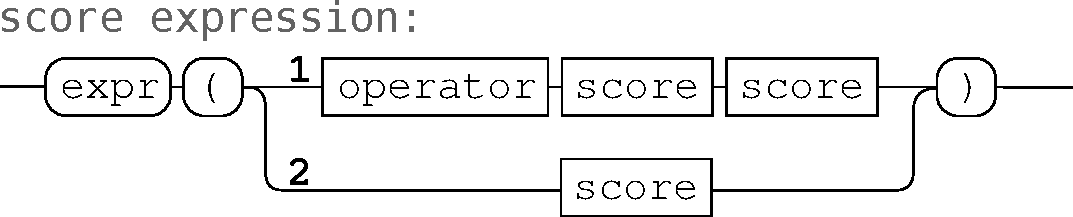
\includegraphics[width=0.9\columnwidth]{imgs/syntax1}
\end{center}

\begin{enumerate}
\item la première forme [1], reflète l'interface des opérateurs : deux partitions sont combinées pour en produire une nouvelle.
\item la deuxième forme [2] défini une expression comme une simple partition, ce qui trouve son utilité pour la duplication d'objets, par exemple pour en fournir des vues différentes (voir section \ref{sample2})
\end{enumerate}

A noter que le mot clé \OSC{expr} est présent pour lever l'ambiguité des parenthèses qui sont également utilisées dans les scripts INScore pour définir des listes de messages.

Les deux formes prennent des \OSC{score} comme arguments. Le système est permissif pour leur type :
\begin{center}
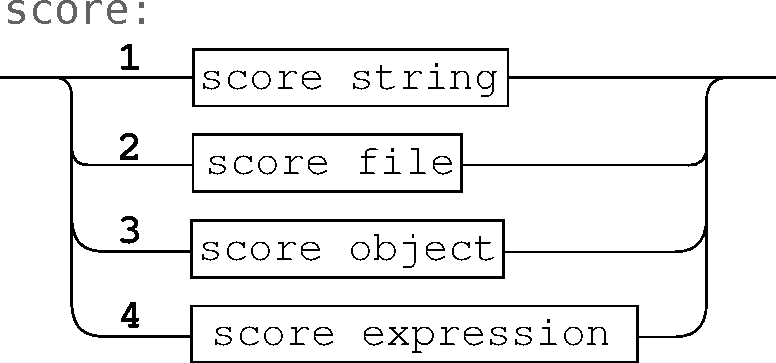
\includegraphics[width=0.7\columnwidth]{imgs/syntax2}
\end{center}

\begin{enumerate}
\item \OSC{score string}: une partition au format GMN ou MusicXML, définit de manière littérale.
\item \OSC{score file}:  fait référence à un fichier au format GMN ou MusicXML. Les chemins d'accès doi-vent suivre les règles définies par INScore et peuvent indiquer des chemins absolus, relatifs ou encore une URL.
\item \OSC{score object}:  fait référence à un objet existant d'INScore en utilisant une adresse OSC relative ou absolue.\\ Cet objet doit être un objet Guido (\OSC{gmn}, ou \OSC{gmnf}), musicxml (\OSC{musicxml}, ou \OSC{musicxmlf}) ou piano-roll (\OSC{pianoroll}, ou \OSC{pianorollf}). \\
Les streams sont également supportés (\OSC{gmnstream}, ou \OSC{pianorollstream}).
\item \OSC{score expression}:  une \sExpr\ peut être utilisée comme argument d'une \sExpr\ (dans ce cas, le mot clé \OSC{expr} est optionnel).
\end{enumerate}

Voici un exemple de \emph{score expression} qui met 2 partitions en parallèle avec 2 partitions en séquence :
\sample{expr( par score.gmn (seq "[c]" score) )}

%==============================================================
\section{Evaluation d'une expression}
\label{evaluationSpec}
Une expression du langage est tout d'abord transformée en une représentation interne en mémoire. Dans un second temps, cette représentation est évaluée pour produire du code au format GMN en sortie, qui est finalement passée à l'objet INScore comme données spécifiques.

%==============================================================
\subsection{Représentation interne d'un expression}

Quand il rencontre une  \sExpr, le parser INScore en crée une représentation mémoire sous forme d'arbre : les feuilles contiennent les arguments et les opérateurs sont des noeuds (Figure \ref{fig:parsing}). Cette forme d'arbre facilite la manipulation et l'évaluation des \sExprs.

\begin{figure}[th]
\centering
\OSC{ expr( \oper{par} \param{score.gmn}  (\oper{seq} \param{"[c]" score})}
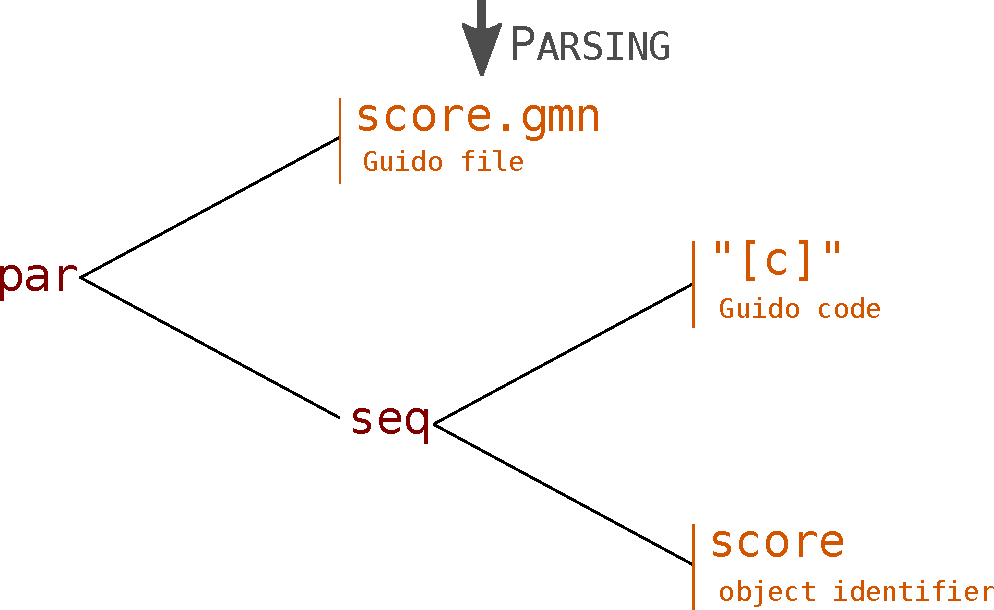
\includegraphics[width=0.8\columnwidth]{imgs/exprParse}
\caption{Représentation d'une expression sous forme d'arbre.
\label{fig:parsing}}
\end{figure}

La représentation sous forme d'arbre est strictement similaire à la version textuelle d'une expression. Le typage des arguments constitue la seule différence : alors que le type des arguments (GMN code, fichier, identificateur ou expression) est implicite dans l'expression textuelle, celui-ci devient explicite dans la représentation mémoire. 

La représentation sous forme d'arbre est stockée avec l'objet correspondant, prête à être évaluée.

%==============================================================
\subsection{Le processus d'évaluation}
Le processus d'évaluation traverse l'arbre d'une expression en utilisant un algorithme de \textit{depth first post-order traversal}, en réduisant chaque noeud à du code GMN (Figure \ref{fig:classicEval}).
L'évaluation d'un noeud dépend de son type:
\begin{itemize}
\item un fichier GMN renvoie son contenu,
\item une chaîne GMN renvoie la chaîne,
\item un fichier MusicXML renvoie son contenu converti au format GMN,
\item une chaîne MusicXML renvoie la chaîne convertie au format GMN,
\item l'identifiant d'object renvoie son code GMN,
\item un opérateur renvoie l'application de l'opérateur à ses arguments.
\end{itemize}

\begin{figure}[th]
\centering
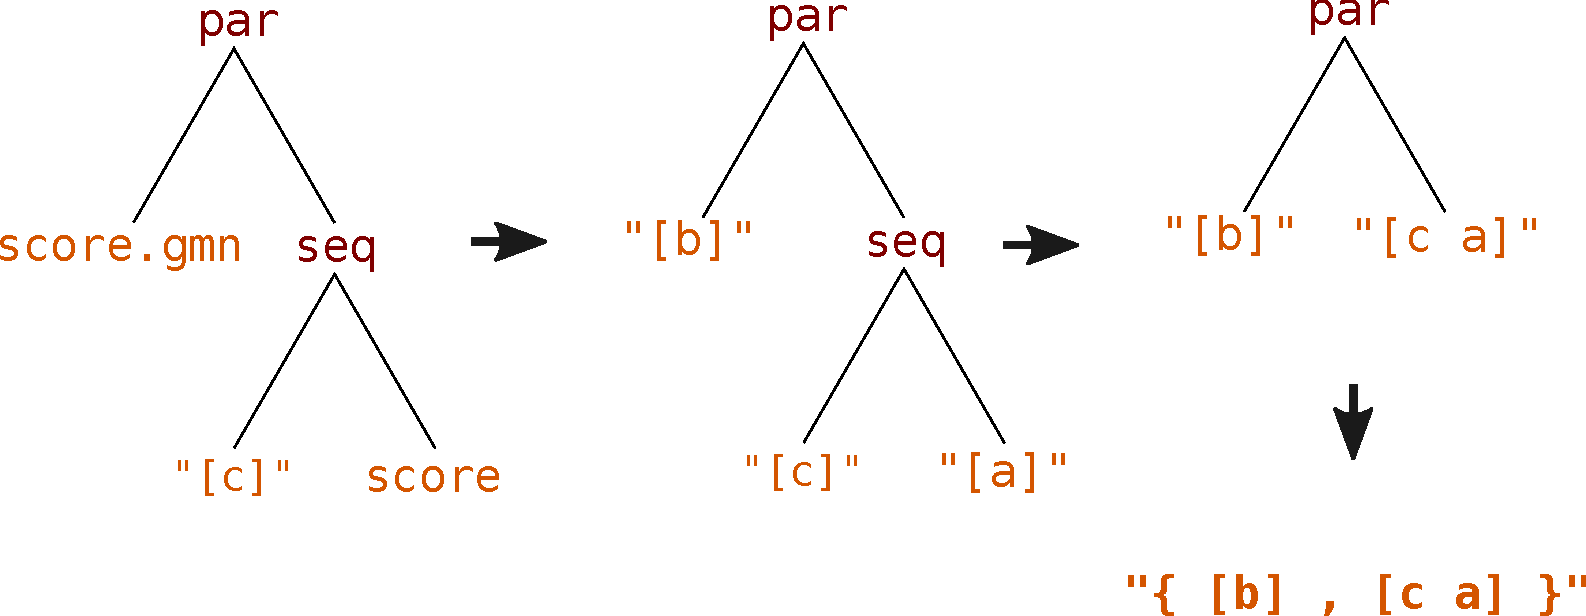
\includegraphics[width=1\columnwidth]{imgs/classicEval}
\caption{Evaluation d'une expression,
où \OSC{score} est défini comme \OSC{[a]}
et \OSC{score.gmn} contient \OSC{[b]}.
\label{fig:classicEval} }
\end{figure}

Ce schéma d'évaluation permet d'éviter les problèmes de récursion (e.g. un objet qui se modifie lui même en utilisant une expression basée sur son propre contenu) puisque l'objet appelant n'est modifié qu'à la fin du processus d'évaluation. 
Une expression est référentiellement transparente : par défaut, chaque argument n'est évalué qu'une fois et sa valeur est alors considérée comme constante.


%==============================================================
\subsection{Evaluation dynamique}

Dans notre cas, la transparence référentielle (qui permet la mémoïsation) peut être une limitation. Par exemple, pour une expression utilisant un stream GMN, on pourrait vouloir maintenir le résultat de l'évaluation de l'expression à jour de l'état actuel du stream. Pour cela, des \emph{arguments variables} ont été introduits en les préfixant du caractère \OSC{\&} : un argument variable est toujours évalué, quelques soit ses valeurs précédentes (Figure \ref{fig:dynamicEval}). Seuls les arguments susceptibles de modification (les fichiers ou les objets INScore) peuvent être déclarés \emph{variables}.

\begin{figure}[th]
\centering
\OSC{ expr( \oper{par} (\oper{seq} \param{score.gmn} \prefix{\&}\param{score}) \\
 \tab\tab\tab\tab (\oper{seq} \param{"[a]" score}) )}
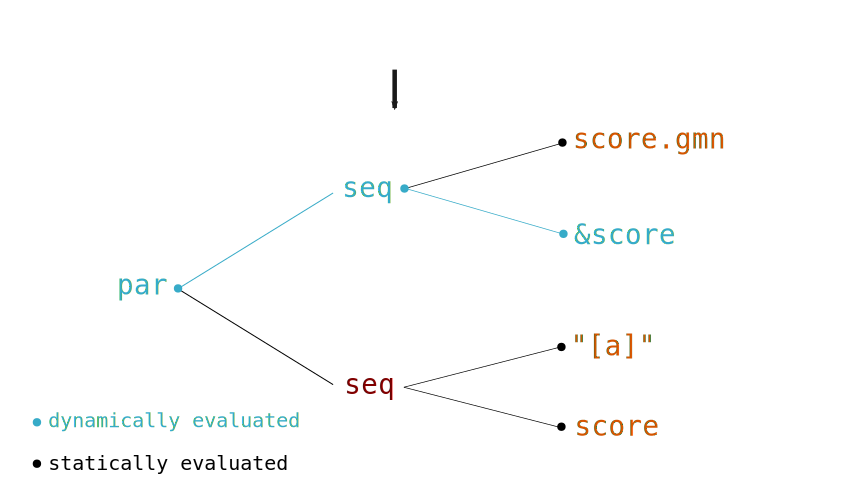
\includegraphics[width=0.9\columnwidth]{imgs/dynamicEval}
\caption{Propagation d'une évaluation dynamique. \OSC{\prefix{\&}\param{score}} est mis à jour avec la valeur courante de \OSC{score} à chaque évaluation, tandis que \OSC{\param{score}} conserve la valeur calculée à la première évaluation. Ainsi, lorsqu'on re-évalue l'expression, la deuxième opération \OSC{\oper{seq}} ne sera pas recalculée. 
}
\label{fig:dynamicEval}
\end{figure}

Un arbre qui contient un argument variable est un \emph{arbre dynamique}. Quand un argument variable est rencontré sur une branche, l'attribut \emph{dynamique} est propagé jusqu'à la racine de l'arbre. Après la première évaluation, seules les parties dynamique d'un arbre sont recalculées. Pour des raisons d'optimisation, le système vérifie que la valeur d'un argument a changé et ne recalcule la branche correspondant que si nécessaire.

L'usage d'arguments variables permet de décrire des expressions comportant des parties variables arbitraires : on peut le voir comme la composition d'une partition symbolique par agrégation de parties statiques et variables.

%==============================================================
\section{L'API des expressions dans INScore}
\label{exprAPI}

Pour une intégration complète des \sExprs, l'implémentation s'appuie sur les fonctionnalités existantes de INScore. De ce fait, les \sExprs\ supportent des URLs comme arguments pour les fichiers, ainsi que les événements d'interaction. La typologie des événements d'interaction a été étendue notamment pour servir les besoins de l'évaluation dynamique (voir section \ref{exprEvents}).

%==============================================================
\subsection{Déclaration d'une expression}
\label{declaringExpr}
Les objets \OSC{gmn} et \OSC{pianoroll} peuvent être définis par des \sExprs\ via une extension du message \OSC{set}.
L'évaluation de l'expression est déclenchée lorsque l'objet cible traite le message \OSC{set}.

\sample{/ITL/scene/score set gmn expr(score.gmn); \\
/ITL/scene/pr set pianoroll expr(\&score);
}

L'exemple précédent crée 2 objets : \OSC{score} qui est une représentation symbolique du fichier GMN \OSC{score.gmn}, et \OSC{pr} qui est une représentation en piano roll de \OSC{score} (évaluée dynamiquement en raison du préfixe  \OSC{\&}).


%==============================================================
\subsection{Messages spécifiques des expressions}
\label{exprMsgs}
Les objets définis par des \sExprs\ acceptent des messages spécifiques :
\begin{itemize}
\item \OSC{reeval}: déclenche la re-évaluation de l'expression. Seules les parties dynamiques sont calculées.
\item \OSC{renew}: déclenche la re-évaluation complète de l'expression, y compris les parties statiques. 
\end{itemize}

Ces messages sont une extension du message \OSC{expr} :
\sample{/ITL/scene/score expr reeval; \\
/ITL/scene/score expr renew;
}

Enfin, l'expression qui définit un objet peut être interrogée avec le message \OSC{get expr} :
\sample{/ITL/scene/score get expr;}

%==============================================================
\subsection{Extension de la typologie des événements}
\label{exprEvents}

Les fonctionnalités d'interaction de INScore sont basées sur l'association d'événements à des listes de messages OSC arbitraires \cite{Fober:13b}. Ces messages sont émis à l'occurence de l'événement correspondant (e.g. un click).
La typologie des événements a été étendue avec un nouvel événement : \OSC{newData}, qui est déclenché par un objet lorsque sa valeur change, soit en raison de la réception d'un message \OSC{set} ou \OSC{reeval}, soit parce que des données ont été écrites dans un objet définit par un stream.

L'association du message \OSC{expr reeval} à l'événement \OSC{newData} permet la réévaluation automatique d'une expression lorsque la valeur d'un objet change :
\sample{/ITL/scene/score set gmn "[a]";\\
/ITL/scene/copy set gmn expr(\&score);\\
/ITL/scene/score watch newData\\   
\hspace*{8mm}(/ITL/scene/copy expr reeval);
}

Dans l'exemple ci-dessus, le changement de valeur de \OSC{score} changera automatiquement la valeur de \OSC{copy}.

Pour gérer les problèmes de boucle infinies, les messages associés à \OSC{newData} sont postés pour la prochaine tâche du temps d'INScore. De ce fait, la mise à jour complète d'une partition après changement de la valeur d'un de ses composants peut s'étendre sur plusieurs tâches du temps (si un objet fait référence à un autre objet, lui-même faisant référence à un autre...) et durant ce processus, la partition peut passer par des états transitoires. De cette manière, les objets faisant référence à eux-même et qui installent un mécanisme de réévaluation automatique ne seront pas bloquants pour le système.


%==============================================================
\section{Composition d'expressions}
\label{composingExpr}
Alors que le langage des expressions permet de composer des partitions symboliques, il permet également de composer les expressions avec le préfixe  \OSC{\prefix{\lowTilde}}. En effet, alors que les arguments \OSC{\param{score}} et \OSC{\prefix{\&}\param{score}} font référence à la valeur de l'objet \OSC{score}, \OSC{\prefix{\lowTilde}\param{score}} fait référence à l'expression qui définit l'objet \OSC{score}. Dans la pratique, et avant la première évaluation, tous les arguments préfixés par \OSC{\prefix{\lowTilde}} sont remplacés par une copie de l'arbre d'expression de l'objet correspondant. Il est ainsi possible de réutiliser des \sExprs\ déjà définies pour construire des expressions plus complexes.

La figure \ref{fig:expandingTree} illustre l'expansion de l'arbre d'expression pour l'exemple ci-dessous.

\sample{/ITL/scene/score set gmn\\
\tab expr(\oper{seq} \param{"[a]"} \prefix{\&}\param{sample});\\
/ITL/scene/score set gmn  \\
\tab expr(\oper{seq} (\oper{seq} \prefix{\lowTilde}\param{score} \param{"[b]"}) \prefix{\lowTilde}\param{score});
}

\begin{figure}[th]
\centering
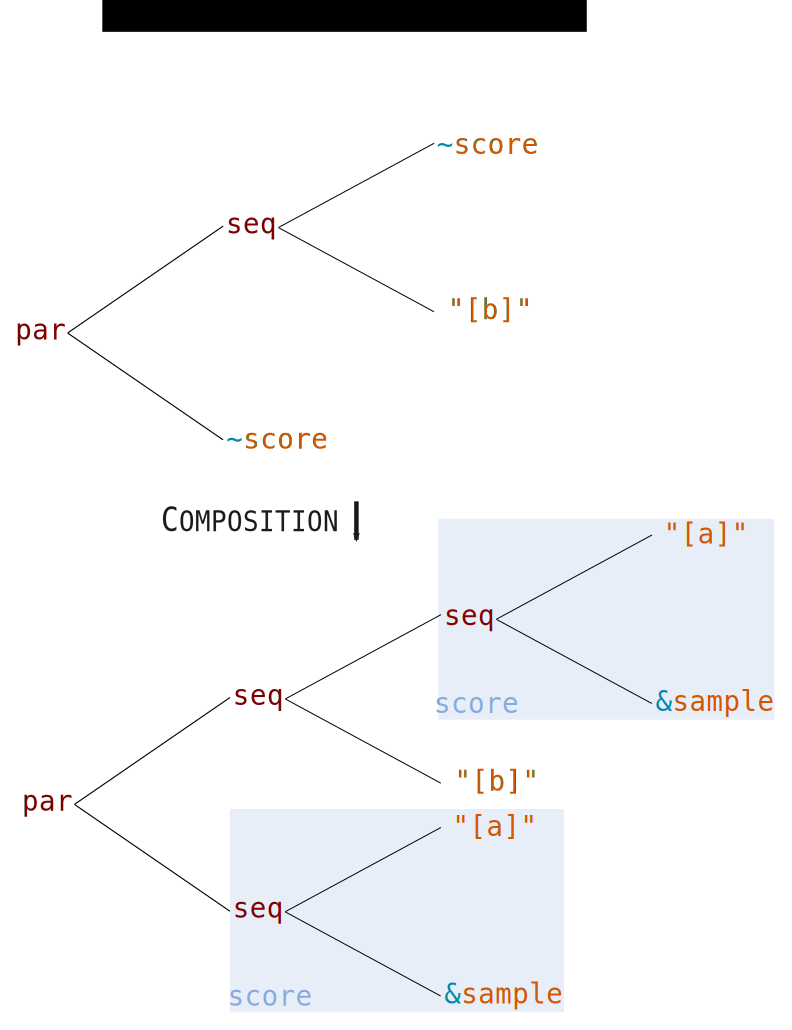
\includegraphics[width=0.9\columnwidth]{imgs/expandingTree}
\caption{Composition d'expressions
\label{fig:expandingTree}}
\end{figure}

%==============================================================
\section{Exemples}
\label{examples}

%==============================================================
\subsection{Canon}

La forme \emph{canon} constitue une structure musicale simple qui peut être facilement décrite par des \sExprs.

Dans l'exemple ci-dessous, la première ligne crée un objet \OSC{score} basé sur un fichier GMN. Il est ensuite transposé à la quinte et une seconde voix est ajoutée avec un délai d'une blanche. Du fait que la transposition à un intervalle spécifique n'est pas une opération de base des opérateurs (l'intervalle de transposition est calculé à partir des 2 partitions), nous combinons \OSC{transpose} avec \OSC{seq} et \OSC{evtail} pour préfixer la partition avec une note qui détermine l'intervalle de transposition, et qui est ensuite supprimée.

\sample{/ITL/scene/score set gmnf score.gmn;\\
\\
\# Transposition de la partition\\
/ITL/scene/canon set gmn\\
\tab expr(evtail\\
\tab\tab(transpose (seq "[c]" score) "[g]")\\
\tab\tab"[a]"\\
\tab);\\
\\
\# Mise en séquence
/ITL/scene/canon set gmn\\
\tab expr(seq score canon);\\
\\
\# Ajout de la second voix décalée d'une blanche\\
/ITL/scene/canon set gmn\\
\tab expr(par canon (seq "[\_/2]" canon));
}
Le résultat est un illustré par la figure \ref{fig:canonFig}
\begin{figure}[th]
\centering
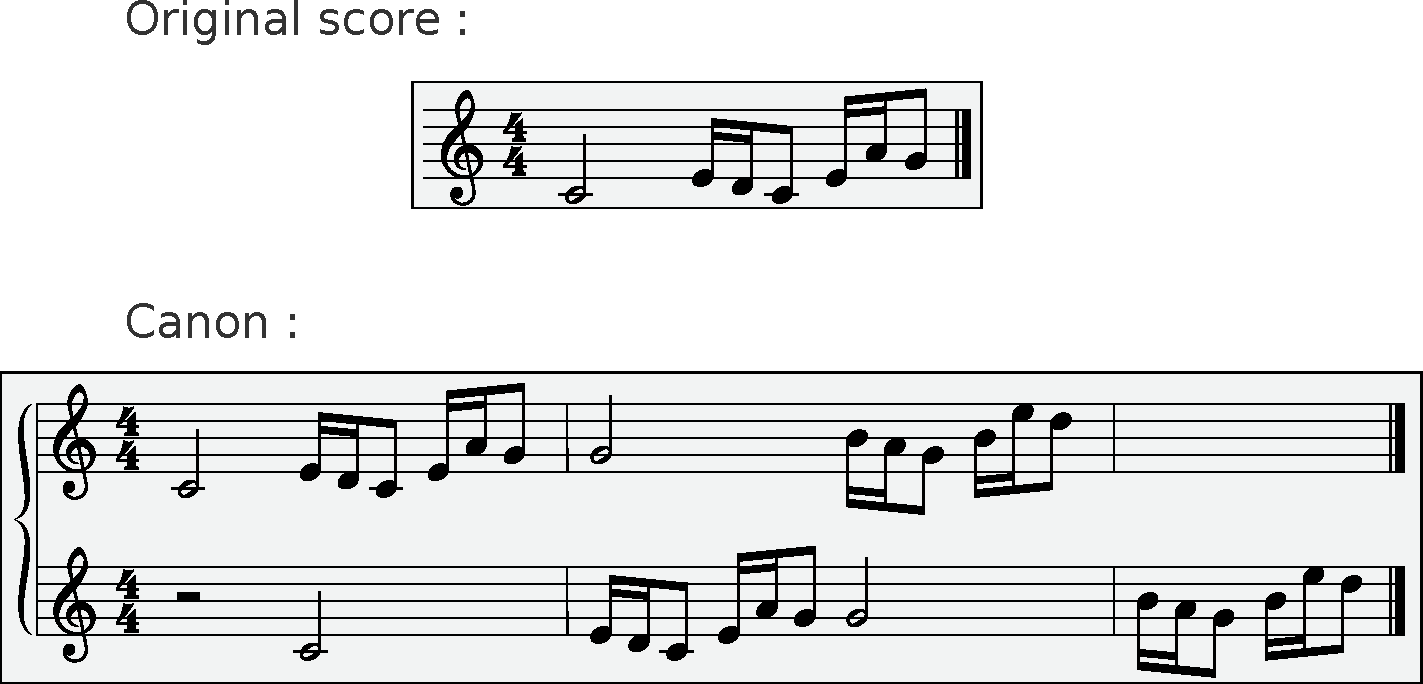
\includegraphics[width=1.\columnwidth]{imgs/exampleCanon}
\caption{Canon
\label{fig:canonFig}}
\end{figure}

%==============================================================
\subsection{Partitions multiformes synchronisées}
\label{sample2}

Les \sExprs\ permettent de dupliquer et de transformer dynamiquement des partitions en les maintenant synchronisées avec l'original.

\sample{/ITL/scene/stream set gmnstream \\
\tab '[$\backslash$meter<"4/4">]';\\
\\
/ITL/saxo/score set gmn \\
\tab expr( evtail\\
\tab \tab (transpose\\
\tab \tab \tab (seq\\
\tab \tab \tab \tab "[e\&1]"\\
\tab \tab \tab \tab \&/ITL/scene/stream )\\
\tab \tab \tab "[c2]" )\\
\tab \tab "[a]"\\
\tab );\\
\\
/ITL/audience/score set pianoroll \\
\tab expr( \&/ITL/scene/stream);\\
\\
/ITL/scene/stream watch newData\\
\tab(/ITL/*/score expr reeval);
}
L'exemple ci-dessus crée 2 copies d'un objet GMN stream. La première est transposée pour le saxophone et la seconde est affichée sous forme de piano roll, en tant que support visuel pour le public. Chaque partition est créée dans des scènes distinctes. La dernière ligne assure la mise à jour des copies lorsque l'objet \OSC{stream} est modifié. Le résultat est présenté par la figure \ref{fig:mutliscoreFig}.

\begin{figure}[th]
\centering
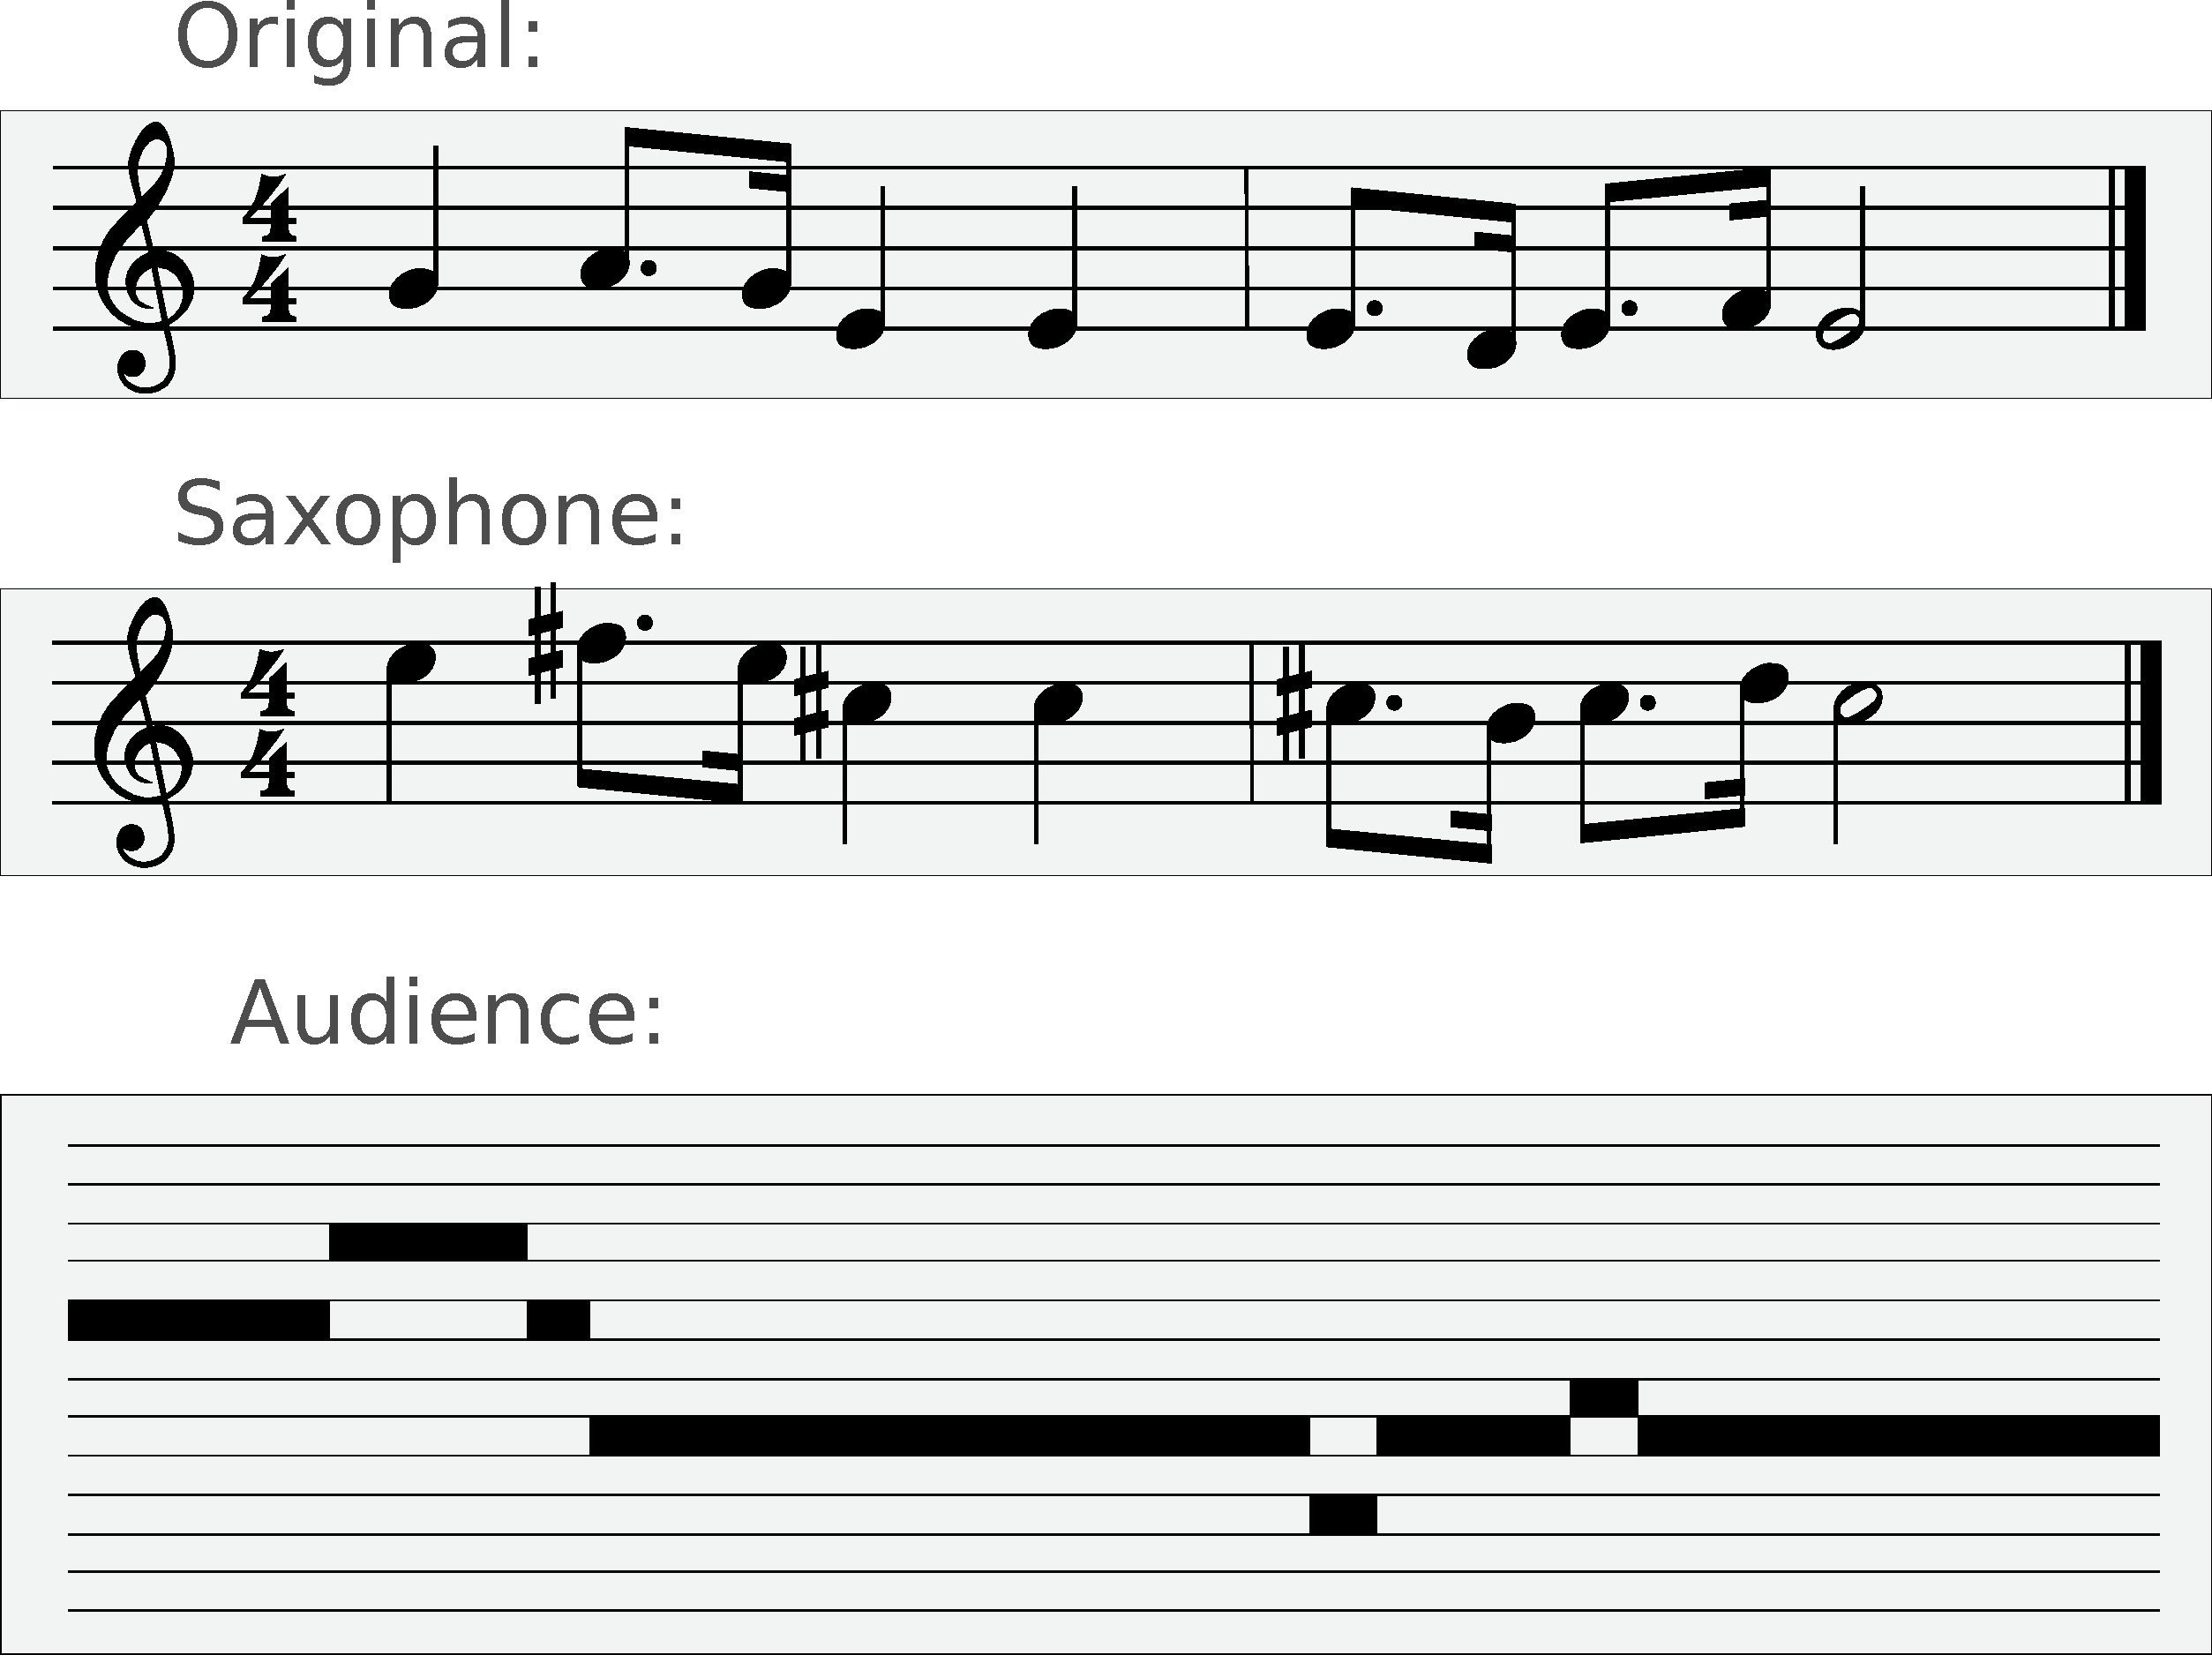
\includegraphics[width=0.95\columnwidth]{imgs/example1}
\caption{Des partitions multi-formes
\label{fig:mutliscoreFig}}
\end{figure}


%------------------------------------------
\subsection{Composer des éléments dynamiques et statiques}\label{sample3}
Cet exemple illustre la composition et la transformation de partitions dynamiques et statiques en temps-réel.
Dans un premier temps, nous créons une partition sous forme de flux (nommée \OSC{stream}), destinée à être écrite en temps réel, et une partition statique (nommée \OSC{static}).
\sample{/ITL/scene/stream set gmnstream \\
\tab \tab '[$\backslash$meter<"4/4">]';\\
/ITL/scene/static set gmn \\
\tab \tab '[$\backslash$meter<"4/4"> g e f a f d c/2]';
}
Dans un deuxième temps, les deux dernières mesures de \OSC{stream} sont extraites et affectées à un nouvel objet nom-mé\OSC{tail}. Du fait que l'opération 'tail' coupe le début de la partition sur la durée de la partition donnée en second argument, la durée de cet argument est exprimée comme la fin de \OSC{stream} après la durée désirée (2 rondes)
L'expression de \OSC{tail} fait usage d'une référence à \OSC{stream} de manière à être mis à jour de ses nouvelles valeurs. 
\sample{/ITL/scene/tail set gmn \\
\tab \tab expr(tail \&stream \\
\tab \tab \tab \tab (tail \&stream '[a*2]')));
}
Le résultat final est obtenu avec les opérations 'par' et 'transpose'. Il inclut une référence à \OSC{tail} mais l'objet \OSC{static} est embarqué statiquement. \OSC{tail} est utilisé comme un objet intermédiaire pour des raisons d'optimisation et facilite par ailleurs la lecture de l'expression. Il peut être caché du rendu final sans affecter le résultat.
\sample{/ITL/scene/score set gmn \\
\tab \tab expr(par \&tail \\
\tab \tab \tab \tab (transpose static \&tail));
}
L'activation du calcul dynamique de la partition fait usage de l'événement \OSC{newData}, surveillé par l'objet \OSC{stream}, qui informe \OSC{tail} et \OSC{score} que leurs expressions doivent être re-évaluées.
\sample{/ITL/scene/stream watch newData \\
\tab \tab (/ITL/scene/part \ expr reeval, \\
\tab \tab \ /ITL/scene/score expr reeval \\
\tab \tab );
}


%==============================================================
\section{Conclusions}

En combinant les opérateurs Guido avec les fonctionnalités d'INScore (API OSC, dimension Web, interactivité...), les \sExprs\ intègrent pleinement la composition de partitions symboliques dans l'environnement interactif des partitions augmentées. Elles étendent le processus d'écriture à la structure musicale et à l'agrégation de partitions par la combinaison de différents matériaux symbolique, incluant d'autres objets de la partition. Elles constituent un jeu d'outils simples pour manipuler des partitions quelle que soit leur origine (fichiers, URLs, streams) ou quelle que soit leur représentation (symbolique, piano roll), et pour concevoir des partitions dynamiques basées sur des compositions arbitraires.

Dans le futur, nous allons étudier l'extension des \sExprs\ à tous les objets d'INScore. Une telle approche - la composition de ressources graphiques arbitraires avec une sémantique musicale - pose des problèmes non triviaux à résoudre. En effet, si les opérations dans le domaine temporel peuvent s'appliquer à n'importe quel objet en raison de leur dimension temporelle commune, les transformations dans le domaine des hauteurs ou dans le domaine du temps structuré (tel que le rythme) impliquent l'extension de la sémantique de l'espace graphique.

\balance
\bibliographystyle{ieeetr}
\bibliography{../interlude}

\end{document}
